% ─── Slide 9a-1: Training Block 0 (vertical two-arch) ─────────────────────────
\begin{frame}[shrink=10]{Our Extension I: Block-wise Calibration \& Propagation}

  \begin{columns}[T]
    \begin{column}{0.36\textwidth}
      \footnotesize
      \textbf{From per-projection to per-block.}\\[0.2em]
      We reconstruct the \emph{whole transformer block}:
      \[
        \mathcal L \;=\; \bigl\| \hat B(\hat x) - B_{\mathrm{FP}}(x^\star) \bigr\|_2^2
      \]
      Each block is trained \emph{one at a time} — here, Decoder Layer 0.

      \vspace{0.5em}
      \textbf{Propagation.}\\[0.2em]
      Input to block $\ell$ is the ADC-quantised output of block $\ell{-}1$.
    \end{column}

    \begin{column}{0.62\textwidth}
      \begin{center}
      \resizebox{!}{0.60\textheight}{%
      \begin{tikzpicture}[
        every node/.style={font=\tiny},
        fbox/.style={draw=mygray!55, dashed, fill=mygray!12, rounded corners=3pt,
                     minimum width=2.5cm, minimum height=0.46cm, align=center},
        tbox/.style={draw=myorange, line width=1.3pt, fill=myorange!22, rounded corners=3pt,
                     minimum width=2.5cm, minimum height=0.46cm, align=center},
        dbox/.style={draw=mygreen!65, fill=mygreen!18, rounded corners=3pt,
                     minimum width=2.5cm, minimum height=0.46cm, align=center},
        garr/.style={-{Latex[length=1.2mm]}, thick, mygray!65},
        tarr/.style={-{Latex[length=1.2mm]}, thick},
        node distance=0.26cm
      ]
        % ── FP Teacher (left) ─────────────────────────────────────────
        \node[font=\tiny, text=mygray!80] (l_x)   at (0,    0)   {$x^\star$};
        \node[fbox, above=0.18cm of l_x]  (l_d0)  {Decoder Layer 0};
        \node[fbox, above=of l_d0]        (l_d1)  {Decoder Layer 1};
        \node[fbox, above=of l_d1]        (l_d2)  {Decoder Layer 2};
        \node[font=\small, text=mygray!70, above=0.10cm of l_d2] (l_dots) {$\cdots$};
        \node[fbox, above=0.10cm of l_dots] (l_dN){Decoding Layer N};
        \node[fbox, above=of l_dN]        (l_rms) {RMS Norm.};
        \node[fbox, above=of l_rms]       (l_log) {Logits};
        \node[fbox, above=of l_log]       (l_sm)  {Softmax};
        \node[fbox, above=of l_sm]        (l_prob){Prob.\ dist.};
        \node[font=\tiny\bfseries, text=mybluedark, above=0.18cm of l_prob] {FP Teacher};

        \draw[garr] (l_x)--(l_d0);
        \foreach \a/\b in {l_d0/l_d1, l_d1/l_d2, l_dN/l_rms,
                           l_rms/l_log, l_log/l_sm, l_sm/l_prob}
          \draw[garr] (\a)--(\b);
        \draw[garr] (l_d2)--(l_dots); \draw[garr] (l_dots)--(l_dN);

        \begin{pgfonlayer}{background}
          \node[inner sep=7pt, draw=mygray!40, dashed, fill=mygray!5,
                rounded corners=7pt, fit=(l_x)(l_prob)] {};
        \end{pgfonlayer}

        % ── Quantized Student (right) ──────────────────────────────────
        \node[font=\tiny, text=mybluedark] (r_x)  at (4.2,  0)   {$\hat x$};
        \node[tbox, above=0.18cm of r_x]  (r_d0)  {Decoder Layer 0};  % TRAINABLE
        \node[fbox, above=of r_d0]        (r_d1)  {Decoder Layer 1};
        \node[fbox, above=of r_d1]        (r_d2)  {Decoder Layer 2};
        \node[font=\small, above=0.10cm of r_d2] (r_dots) {$\cdots$};
        \node[fbox, above=0.10cm of r_dots] (r_dN){Decoding Layer N};
        \node[fbox, above=of r_dN]        (r_rms) {RMS Norm.};
        \node[fbox, above=of r_rms]       (r_log) {Logits};
        \node[fbox, above=of r_log]       (r_sm)  {Softmax};
        \node[fbox, above=of r_sm]        (r_prob){Prob.\ dist.};
        \node[font=\tiny\bfseries, text=mybluedark, above=0.18cm of r_prob] {Student};

        \draw[tarr] (r_x)--(r_d0);
        \foreach \a/\b in {r_d0/r_d1, r_d1/r_d2, r_dN/r_rms,
                           r_rms/r_log, r_log/r_sm, r_sm/r_prob}
          \draw[garr] (\a)--(\b);
        \draw[garr] (r_d2)--(r_dots); \draw[garr] (r_dots)--(r_dN);

        % Green highlight: trainable block
        \begin{pgfonlayer}{background}
          \node[inner sep=5pt, draw=myorange!60, fill=myorange!8, rounded corners=5pt,
                fit=(r_d0)] (rb0) {};
        \end{pgfonlayer}

        % Braces
        \draw[decorate, decoration={brace, amplitude=3pt}, myorange]
          (rb0.north east) -- (rb0.south east)
          node[midway, right=4pt, font=\tiny, text=myorange] {trainable};
        \draw[decorate, decoration={brace, amplitude=3pt}, mygray!65]
          (r_prob.north east) -- (r_d1.south east)
          node[midway, right=4pt, font=\tiny, text=mygray] {frozen};

        % Loss arrow at Decoder 0 level
        \draw[{Latex[length=1.2mm]}-{Latex[length=1.2mm]}, thick, myred!75]
          (l_d0.east) -- node[above, font=\tiny, fill=white, inner sep=1pt]
          {$\mathcal{L}$} (r_d0.west);

      \end{tikzpicture}}
      \end{center}
    \end{column}
  \end{columns}
\end{frame}

% ─── Slide 9a-2: Training Block 1 (vertical two-arch) ─────────────────────────
\begin{frame}[shrink=10]{Our Extension I: Block-wise Calibration \& Propagation}

  \begin{columns}[T]
    \begin{column}{0.36\textwidth}
      \footnotesize
      \textbf{From per-projection to per-block.}\\[0.2em]
      We reconstruct the \emph{whole transformer block}:
      \[
        \mathcal L \;=\; \bigl\| \hat B(\hat x) - B_{\mathrm{FP}}(x^\star) \bigr\|_2^2
      \]
      Now \textbf{Decoder Layer 1}. Its input is the \alert{ADC-quantised output of Layer 0}.

      \vspace{0.5em}
      \textbf{Propagation.}\\[0.2em]
      Error accumulates \emph{the same way at train time and at inference}.
    \end{column}

    \begin{column}{0.62\textwidth}
      \begin{center}
      \resizebox{!}{0.60\textheight}{%
      \begin{tikzpicture}[
        every node/.style={font=\tiny},
        fbox/.style={draw=mygray!55, dashed, fill=mygray!12, rounded corners=3pt,
                     minimum width=2.5cm, minimum height=0.46cm, align=center},
        tbox/.style={draw=myorange, line width=1.3pt, fill=myorange!22, rounded corners=3pt,
                     minimum width=2.5cm, minimum height=0.46cm, align=center},
        dbox/.style={draw=mygreen!65, fill=mygreen!18, rounded corners=3pt,
                     minimum width=2.5cm, minimum height=0.46cm, align=center},
        garr/.style={-{Latex[length=1.2mm]}, thick, mygray!65},
        tarr/.style={-{Latex[length=1.2mm]}, thick},
        node distance=0.26cm
      ]
        % ── FP Teacher (left) — identical to slide 1 ──────────────────
        \node[font=\tiny, text=mygray!80] (l_x)   at (0,    0)   {$x^\star$};
        \node[fbox, above=0.18cm of l_x]  (l_d0)  {Decoder Layer 0};
        \node[fbox, above=of l_d0]        (l_d1)  {Decoder Layer 1};
        \node[fbox, above=of l_d1]        (l_d2)  {Decoder Layer 2};
        \node[font=\small, text=mygray!70, above=0.10cm of l_d2] (l_dots) {$\cdots$};
        \node[fbox, above=0.10cm of l_dots] (l_dN){Decoding Layer N};
        \node[fbox, above=of l_dN]        (l_rms) {RMS Norm.};
        \node[fbox, above=of l_rms]       (l_log) {Logits};
        \node[fbox, above=of l_log]       (l_sm)  {Softmax};
        \node[fbox, above=of l_sm]        (l_prob){Prob.\ dist.};
        \node[font=\tiny\bfseries, text=mybluedark, above=0.18cm of l_prob] {FP Teacher};

        \draw[garr] (l_x)--(l_d0);
        \foreach \a/\b in {l_d0/l_d1, l_d1/l_d2, l_dN/l_rms,
                           l_rms/l_log, l_log/l_sm, l_sm/l_prob}
          \draw[garr] (\a)--(\b);
        \draw[garr] (l_d2)--(l_dots); \draw[garr] (l_dots)--(l_dN);

        \begin{pgfonlayer}{background}
          \node[inner sep=7pt, draw=mygray!40, dashed, fill=mygray!5,
                rounded corners=7pt, fit=(l_x)(l_prob)] {};
        \end{pgfonlayer}

        % ── Quantized Student (right) ──────────────────────────────────
        \node[font=\tiny, text=mybluedark] (r_x)  at (4.2,  0)   {$\hat x$};
        \node[dbox, above=0.18cm of r_x]  (r_d0)  {Decoder Layer 0};  % DONE
        \node[tbox, above=of r_d0]        (r_d1)  {Decoder Layer 1};  % TRAINABLE
        \node[fbox, above=of r_d1]        (r_d2)  {Decoder Layer 2};
        \node[font=\small, above=0.10cm of r_d2] (r_dots) {$\cdots$};
        \node[fbox, above=0.10cm of r_dots] (r_dN){Decoding Layer N};
        \node[fbox, above=of r_dN]        (r_rms) {RMS Norm.};
        \node[fbox, above=of r_rms]       (r_log) {Logits};
        \node[fbox, above=of r_log]       (r_sm)  {Softmax};
        \node[fbox, above=of r_sm]        (r_prob){Prob.\ dist.};
        \node[font=\tiny\bfseries, text=mybluedark, above=0.18cm of r_prob] {Student};

        \draw[garr] (r_x)--(r_d0);
        \draw[garr] (r_d0)--(r_d1);
        \foreach \a/\b in {r_d1/r_d2, r_dN/r_rms,
                           r_rms/r_log, r_log/r_sm, r_sm/r_prob}
          \draw[garr] (\a)--(\b);
        \draw[garr] (r_d2)--(r_dots); \draw[garr] (r_dots)--(r_dN);

        % Green highlights
        \begin{pgfonlayer}{background}
          \node[inner sep=5pt, draw=mygreen!60, fill=mygreen!8, rounded corners=5pt,
                fit=(r_d0)] (rd0_bg) {};
          \node[inner sep=5pt, draw=myorange!60, fill=myorange!8, rounded corners=5pt,
                fit=(r_d1)] (rb1) {};
        \end{pgfonlayer}

        % Braces
        \draw[decorate, decoration={brace, amplitude=3pt}, mygreen!70]
          (rd0_bg.north east) -- (rd0_bg.south east)
          node[midway, right=4pt, font=\tiny, text=mygreen!70!black] {done\,$\checkmark$};
        \draw[decorate, decoration={brace, amplitude=3pt}, myorange]
          (rb1.north east) -- (rb1.south east)
          node[midway, right=4pt, font=\tiny, text=myorange] {trainable};
        \draw[decorate, decoration={brace, amplitude=3pt}, mygray!65]
          (r_prob.north east) -- (r_d2.south east)
          node[midway, right=4pt, font=\tiny, text=mygray] {frozen};

        % Loss arrow at Decoder 1 level
        \draw[{Latex[length=1.2mm]}-{Latex[length=1.2mm]}, thick, myred!75]
          (l_d1.east) -- node[above, font=\tiny, fill=white, inner sep=1pt]
          {$\mathcal{L}$} (r_d1.west);

      \end{tikzpicture}}
      \end{center}
    \end{column}
  \end{columns}
\end{frame}

% ─── Slide 9b: α-mixed objective ─────────────────────────────────────────────
\begin{frame}[shrink=10]{Our Extension I: $\alpha$-Mixed Objective}

  \begin{columns}[T]
    \begin{column}{0.50\textwidth}
      \footnotesize
      \textbf{From per-projection to per-block.}\\[0.2em]
      FlatQuant calibrates each linear layer separately (MSE on its output). We reconstruct the \emph{whole transformer block}:
      \[
        \mathcal L \;=\; \bigl\| \hat B\!\left(\hat x\right) - B_{\mathrm{FP}}(x^\star) \bigr\|_2^2
      \]
      Gradients flow through q/k/v $\to$ attn $\to$ o $\to$ gate/up $\to$ down.

      \vspace{0.5em}
      \textbf{$\alpha$-mixed objective.}\\[0.2em]
      Feed both FP and ADC inputs through the student block in one step:
      \[
        \mathcal L(\alpha) \;=\; (1{-}\alpha)\,\mathcal L_{\mathrm{FP}} \;+\; \alpha\,\mathcal L_{\mathrm{ADC}}
      \]
      \scriptsize
      $\alpha{=}0$: clean — easy to fit, ignores ADC noise.\\
      $\alpha{=}1$: realistic — matches inference but hard to optimise (noisy grads).\\
      $\alpha{=}0.5$: \emph{both} signals at once.
    \end{column}

    \begin{column}{0.48\textwidth}
      \begin{center}
      \resizebox{\linewidth}{!}{%
      \begin{tikzpicture}[
        every node/.style={font=\scriptsize},
        dq/.style={draw=mybluedark, rounded corners=2pt, fill=myblue!20,
                   minimum width=1.2cm, minimum height=0.50cm, align=center},
        tile/.style={draw=mybluedark, rounded corners=2pt, fill=mybluedark!12,
                     text=mybluedark, minimum width=1.6cm, minimum height=0.65cm, align=center},
        adc/.style={draw=myorange, line width=1.2pt, rounded corners=2pt,
                    fill=myorange!25, minimum width=1.0cm, minimum height=0.50cm, align=center},
        tbox/.style={draw=mygray!55, rounded corners=4pt, fill=mygray!10,
                     minimum width=2.6cm, minimum height=0.65cm, align=center},
        arr/.style={-{Latex[length=1.3mm]}, thick}
      ]
        % ── Student: ADC pipeline ────────────────────────────────────
        \node (w)  at (0,   0.8) {$w$};
        \node[dq]  (qw) at (1.5,  0.8) {Digital\\quantiser};
        \node (wb) at (3.0,  0.8) {$\hat w$};
        \node (x)  at (0,  -0.8) {$x$};
        \node[dq]  (qx) at (1.5, -0.8) {Digital\\quantiser};
        \node (xb) at (3.0, -0.8) {$\hat x$};

        \draw[arr] (w)--(qw);  \draw[arr] (qw)--(wb);
        \draw[arr] (x)--(qx);  \draw[arr] (qx)--(xb);

        \node[tile] (T) at (4.6, 0) {Analog IMC\\$y{=}\langle\hat w,\hat x\rangle$};
        \draw[arr] (wb) -- (T.north west);
        \draw[arr] (xb) -- (T.south west);

        \node (y)  at (6.0, 0) {$y$};
        \draw[arr] (T)--(y);

        \node[adc] (A) at (7.1, 0) {ADC\\$\lfloor y/\delta\rfloor$};
        \draw[arr] (y)--(A);

        \node (yh) at (8.2, 0) {$\hat y$};
        \draw[arr] (A)--(yh);

        % Gray box: Student
        \begin{pgfonlayer}{background}
          \node[inner sep=9pt, draw=mygray!50, fill=mygray!7, rounded corners=8pt,
                fit=(w)(qw)(wb)(x)(qx)(xb)(T)(y)(A)(yh)] (sbox) {};
        \end{pgfonlayer}
        \node[font=\scriptsize\bfseries, text=mygray!80,
              anchor=south west, xshift=4pt, yshift=2pt] at (sbox.north west) {Student};

        % ── Teacher ──────────────────────────────────────────────────
        \node[tbox] (teach) at (7.1, -2.5)
          {Teacher:\enspace $y^\star = \langle w,\, x\rangle$};
        \node[font=\scriptsize\bfseries, text=mygray!80,
              anchor=south west, xshift=4pt, yshift=2pt] at (teach.north west) {Teacher};

        % ── L_FP: teacher ↔ y (pre-ADC, blue) ───────────────────────
        \draw[{Latex[length=1.3mm]}-{Latex[length=1.3mm]}, thick, myblue!80]
          (teach.north west) |-
          node[pos=0.75, left=2pt, font=\scriptsize, text=myblue, fill=white, inner sep=1pt]
          {$\mathcal{L}_{\rm FP}$} (y.south);

        % ── L_ADC: teacher ↔ ŷ (post-ADC, orange) ───────────────────
        \draw[{Latex[length=1.3mm]}-{Latex[length=1.3mm]}, thick, myorange!90]
          (teach.north east) |-
          node[pos=0.75, right=2pt, font=\scriptsize, text=myorange, fill=white, inner sep=1pt]
          {$\mathcal{L}_{\rm ADC}$} (yh.south);

      \end{tikzpicture}}

      \vspace{0.3em}
      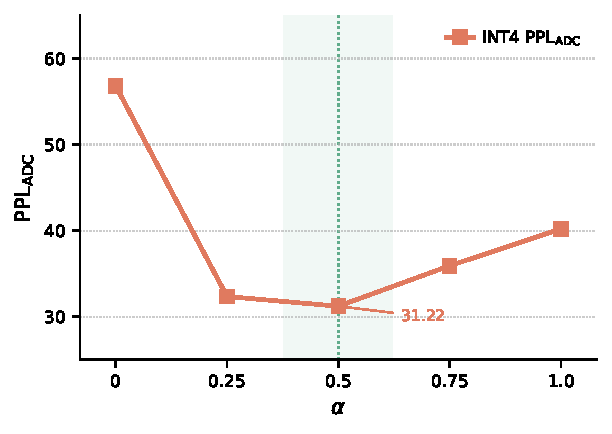
\includegraphics[width=0.78\linewidth]{figs/plot_alpha_sweep.pdf}
      \end{center}
    \end{column}
  \end{columns}

\end{frame}

% ─── Slide 9c: Full summary slide ────────────────────────────────────────────
\begin{frame}[shrink=10]{Our Extension I: Block-wise Calibration \& $\alpha$-Mix}

  \begin{columns}[T]
    \begin{column}{0.5\textwidth}
      \footnotesize
      \textbf{From per-projection to per-block.}\\[0.2em]
      FlatQuant calibrates each linear layer separately (MSE on its output). We reconstruct the \emph{whole transformer block}:
      \[
        \mathcal L \;=\; \bigl\| \hat B\!\left(\hat x\right) - B_{\mathrm{FP}}(x^\star) \bigr\|_2^2
      \]
      Gradients flow through q/k/v $\to$ attn $\to$ o $\to$ gate/up $\to$ down, so \alert{ADC error from earlier projections is seen by later ones during optimisation}.

      \vspace{0.3em}
      \textbf{Propagation across blocks.}\\[0.2em]
      Input to block $\ell$ is the ADC-quantised output of block $\ell{-}1$, \emph{not} its FP teacher activation. The error accumulates \emph{the same way at train time and at inference}.
    \end{column}

    \begin{column}{0.48\textwidth}
      \footnotesize
      \textbf{$\alpha$-mixed objective.}\\[0.2em]
      Feed both FP and ADC inputs through the student block in one step:
      \[
        \mathcal L(\alpha) \;=\; (1{-}\alpha)\,\mathcal L_{\mathrm{FP}} \;+\; \alpha\,\mathcal L_{\mathrm{ADC}}
      \]
      \scriptsize $\alpha{=}0$: clean — easy to fit, ignores ADC noise.\\
      $\alpha{=}1$: realistic — matches inference but hard to optimise (noisy grads).\\
      $\alpha{=}0.5$: \emph{both} signals at once.

      \vspace{0.3em}
      \begin{center}
      \scriptsize
      \renewcommand{\arraystretch}{1.15}
      \begin{tabular}{@{}c c c@{}}
        \toprule
        $\alpha$ & INT8 \adcppl{} & INT4 \adcppl{} \\
        \midrule
        0.0 & 28.86 & 38.5 \\
        \alert{0.5} & \best{14.41} & \best{27.56} \\
        1.0 & 19.70 & 31.8 \\
        \bottomrule
      \end{tabular}
      \end{center}
    \end{column}
  \end{columns}

  \vspace{0.4em}
  \begin{exampleblock}{What this buys us (INT8)}
    \small $\adcppl{}\; 28.86 \to \mathbf{14.41}$ just from switching the loss from per-projection MSE to block $\alpha$-mix. No extra parameters.
  \end{exampleblock}

\end{frame}
